\documentclass[conference]{IEEEtran}
\IEEEoverridecommandlockouts

\usepackage{cite}
\usepackage{amsmath,amssymb,amsfonts}
\usepackage{graphicx}
\usepackage{textcomp}
\usepackage{xcolor}
\usepackage{booktabs}

\begin{document}

\title{Image Corruption Robustness of Lightweight CNNs under Limited Compute}

\author{
\IEEEauthorblockN{Manuk Manukyan}
\IEEEauthorblockA{
American University of Armenia\\
Yerevan, Armenia\\
manuk\_manukyan@edu.aua.am}
\and
\IEEEauthorblockN{Davit Ghazaryan}
\IEEEauthorblockA{
American University of Armenia\\
Yerevan, Armenia\\
dghazaryan@aua.am}
}

\maketitle

\begin{abstract}
Convolutional neural networks achieve strong accuracy on standard image classification benchmarks, yet performance often deteriorates sharply when inputs are affected by realistic degradations such as noise, blur, compression artifacts, resolution loss, and brightness shifts. Most robustness research has focused on large-scale datasets, expensive training pipelines, or heavy model families --- leaving open a practical question about how lightweight CNNs behave under constrained training conditions. This study trains three lightweight architectures from scratch on CIFAR-10 and evaluates them under three training strategies --- no augmentation, standard augmentation, and degradation-aware augmentation --- across 25 corruption conditions spanning five types and five severity levels. Clean accuracy ranges from 80.0\% to 86.1\% across models under unaugmented training. Degradation-aware augmentation raises mean corruption accuracy by 17--25 percentage points over unaugmented training, reaching 70.7\%, 66.0\%, and 77.5\% for the three architectures respectively, with negligible clean accuracy cost on two of three models. Standard augmentation, despite improving clean accuracy to as high as 88.7\%, provides no meaningful robustness benefit --- mean accuracy differences from the unaugmented baseline fall below 2 percentage points across all models and corruption types. A simple four-layer CNN without batch normalization outperforms a residual network under Gaussian noise without augmentation, demonstrating that architectural sophistication does not automatically confer robustness. The results indicate that training strategy matters more than model design for corruption robustness in constrained settings, and that standard augmentation should not be assumed to address input distribution shift.
\end{abstract}

\section{Introduction}

Image classification systems are often developed and reported under conditions that are cleaner than those encountered in practice. Benchmark datasets typically contain well-formed images with limited distortion, stable lighting, and minimal compression artifacts. Real inputs rarely look like that. Images collected by phones, surveillance cameras, embedded devices, or low-bandwidth pipelines are frequently degraded by sensor noise, blur, reduced resolution, compression, or poor illumination. A classifier that performs well on clean benchmark data may therefore become unreliable once image quality begins to deteriorate.

Recent work has made this problem difficult to ignore. Corruption benchmarks such as ImageNet-C and ImageNet-P showed that modern image classifiers remain surprisingly fragile under common, non-adversarial degradations, and that improvements in clean accuracy do not necessarily yield comparable gains in robustness~\cite{hendrycks2019}. That line of work helped shift attention away from robustness as a narrow adversarial question and toward robustness as a broader issue of stability under realistic distribution shift. At roughly the same time, work on model representations suggested that these failures are not accidental --- CNNs trained on standard datasets were shown to rely heavily on texture cues, and increasing shape bias produced improved robustness to distortions~\cite{geirhos2019}.

Training-time augmentation quickly became one of the main responses to this weakness. Methods such as AugMix demonstrated that corruption robustness can be improved substantially without redesigning the network architecture~\cite{hendrycks2020}. Yet later studies showed these gains are often conditional. Robustness improvements tend to be strongest when the corruptions encountered at test time resemble the transformations used during training, while transfer to perceptually dissimilar corruptions can be much weaker~\cite{mintun2021}. Frequency-based analyses reached a similar conclusion from another angle, showing that augmentation can improve robustness to one family of shifts while reducing it for another~\cite{yin2019}.

Although the literature has clarified the main contours of corruption robustness, one practical setting remains underexplored. Much of the influential work has been developed around large-scale datasets, substantial compute budgets, and model families that are not especially constrained~\cite{hendrycks2019,hendrycks2020,mintun2021,geirhos2019,rusak2020,yin2019}. Lightweight CNNs trained on small images are common in edge scenarios, teaching environments, and resource-constrained experimentation, but their robustness behavior has not been studied as systematically under tightly controlled compute limits. In that regime, low-cost interventions matter more, and it becomes important to ask not only whether robustness can be improved, but how much improvement is realistically achievable without expensive pipelines.

This project addresses that gap through a controlled study of lightweight CNN architectures trained on CIFAR-10. The focus is on realistic image degradations that are easy to motivate operationally: Gaussian noise, blur, JPEG compression, resolution reduction, and brightness changes. Three training strategies are compared under identical experimental conditions. The study is guided by three research questions:
\begin{enumerate}
    \item How does CNN performance change as image quality degrades across corruption types and severity levels?
    \item To what extent do low-cost training strategies improve robustness relative to standard training?
    \item Does degradation-aware augmentation provide consistent gains across all corruption types, or are improvements selective?
\end{enumerate}

The contribution is empirical rather than algorithmic. Rather than proposing a new robustness method, the goal is a reproducible analysis of robustness trends and trade-offs in a constrained setting --- one where architecture choice, augmentation cost, and the limits of low-cost interventions are all part of the practical question.

\section{Literature Review}

Robust image classification remains harder than standard benchmark accuracy would suggest. Models that score well on clean test sets can become brittle once images are degraded by noise, blur, or small distribution shifts that are routine outside the lab. Early robustness work in vision focused heavily on adversarial perturbations, but that line of research does not fully capture the kinds of degradations that appear in deployed systems. Common corruptions are less pathological and often more operationally relevant. They expose a different weakness: modern CNNs may generalize well within a benchmark distribution while failing to preserve stable predictions when image quality changes in ordinary ways~\cite{hendrycks2019}.

A major step in making that weakness visible was the introduction of corruption benchmarks such as ImageNet-C and ImageNet-P~\cite{hendrycks2019}. Those benchmarks changed the discussion from anecdotal examples of failure to a controlled evaluation setting with standardized corruption types and severity levels. One of the more striking findings was that robustness did not improve much as architectures moved from older models to more modern residual networks~\cite{hendrycks2019}. Clean-data progress did not automatically translate into meaningful gains in corruption robustness --- a result that matters because it separates two goals still often conflated in practice.

Part of the answer to why CNNs fail so predictably lies in the visual cues they rely on. Geirhos et al.\ showed that ImageNet-trained CNNs are strongly biased toward texture rather than shape~\cite{geirhos2019}. Under texture-shape cue conflict, predictions were driven primarily by local surface statistics, not by global object structure. That explains why corruptions that disrupt fine-scale texture can have outsized effects on classifier output. When the same architecture was trained on Stylized-ImageNet, shape bias increased and robustness improved across a wide range of distortions~\cite{geirhos2019}. Robustness is therefore not just a property of architecture depth or parameter count --- it is tied to the kind of representation a training pipeline encourages the model to learn.

A related explanation emerges from frequency-domain analyses. Yin et al.\ examined corruption robustness from a Fourier perspective and found that gains from augmentation are often selective~\cite{yin2019}. Gaussian noise augmentation improved robustness to high-frequency corruptions, yet the same procedure could reduce robustness to low-frequency shifts such as contrast changes. In practice, that means headline improvements on a benchmark average can hide meaningful trade-offs across corruption types~\cite{yin2019}.

These observations motivated significant work on training-time augmentation. AugMix became one of the most influential approaches because it improved both corruption robustness and uncertainty estimation while adding only modest overhead to standard training~\cite{hendrycks2020}. Results showed that robustness could be improved substantially with data processing alone, without redesigning the model or changing the loss function~\cite{hendrycks2020}. That finding suggested that at least part of the robustness problem reflects how models are exposed to image variability during training.

Augmentation-based robustness has proven less universal than early benchmark gains might imply, however. Mintun et al.\ showed that robustness improvements correlate strongly with perceptual similarity between training-time and test-time perturbations~\cite{mintun2021}. When evaluation corruptions were sampled to be dissimilar from those in training, performance degraded markedly even for models trained with recent robustness augmentations~\cite{mintun2021}. Many methods are good at interpolation around the perturbation families they have seen, but much less reliable under extrapolation.

Rusak et al.\ showed that a simple strategy --- carefully tuned additive Gaussian and Speckle noise during training --- can generalize well to a diverse set of unseen corruptions~\cite{rusak2020}. Robustness gains do not always require elaborate pipelines. At the same time, Yin et al.\ caution that such gains are rarely free of trade-offs: noise-based augmentation tends to help against high-frequency distortions while potentially hurting on low-frequency shifts~\cite{yin2019,rusak2020}.

Across this literature, a consistent picture has emerged. Common corruption benchmarks established that CNNs remain fragile under realistic degradations even when clean accuracy is high~\cite{hendrycks2019}. Representation-level work tied that fragility to texture bias~\cite{geirhos2019}. Augmentation studies showed robustness can be improved, but conditionally on the types of corruptions seen during training~\cite{hendrycks2020,mintun2021,rusak2020,yin2019}.

Most influential studies were developed in large-scale experimental settings centered on ImageNet with substantial computational budgets~\cite{hendrycks2019,hendrycks2020,mintun2021,geirhos2019,rusak2020}. Those papers are invaluable for identifying the problem and the main solution families, but they leave open a practical question: what robustness patterns remain when the setting is deliberately constrained? The present study is positioned within that narrower but practically important space.

\section{Methodology}

\subsection{Dataset and Preprocessing}

All experiments use CIFAR-10, a standard benchmark of 60,000 RGB images at $32{\times}32$ resolution across ten classes, with a fixed split of 50,000 training and 10,000 test images. CIFAR-10 was chosen for two reasons: the $32{\times}32$ resolution makes full training feasible on a single consumer GPU in under an hour per model, and the dataset is sufficiently well-established in the robustness literature that results are interpretable in the context of prior work. Images are normalized using the dataset channel means $(0.4914, 0.4822, 0.4465)$ and standard deviations $(0.2023, 0.1994, 0.2010)$. No test-time preprocessing beyond normalization is applied in any condition.

\subsection{Architectures}

Three lightweight CNNs are trained from scratch. The architectures were chosen to differ in specific, theoretically motivated ways rather than to maximize clean accuracy. Each model isolates a different combination of design choices, making the robustness comparison interpretable rather than confounded.

\textbf{BaselineCNN} is a four-layer sequential network with 32, 32, 64, and 64 filters, max pooling after every two convolutional layers, and fully connected layers mapping $64{\times}8{\times}8 = 4096$ features to 128 then to 10 outputs. No batch normalization is used anywhere in the network. Dropout ($p = 0.5$) is applied before the final layer. At approximately 560K parameters, it serves as the minimal reference point --- a network with no modern regularization techniques beyond dropout.

\textbf{LightweightResNet} is a compact residual network with an initial convolution followed by two residual blocks (32 and 64 filters). Batch normalization is applied after every convolution, and skip connections handle dimension changes between blocks. Global average pooling replaces the spatial flattening used in BaselineCNN, reducing the final representation to 64 values before a single linear output layer. This gives roughly 180K parameters --- the smallest of the three models. The key architectural differences from BaselineCNN are the residual connections, batch normalization, and global average pooling, all of which are expected to improve generalization.

\textbf{WiderCNN} uses four convolutional layers with 64, 64, 128, and 128 filters, batch normalization after every convolution, and a larger fully connected head mapping $128{\times}8{\times}8 = 8192$ features to 256 then to 10 outputs with dropout ($p = 0.5$). At approximately 2.1M parameters, it is the highest-capacity model. Unlike LightweightResNet, it has no residual connections --- the design isolates the effect of increased capacity and batch normalization from the effect of skip connections.

\subsection{Design Justification}

The three architectures were selected to answer a specific question: does robustness under corruption track with architectural sophistication, or is the relationship more complicated? BaselineCNN provides a minimal baseline with no batch normalization and no skip connections. LightweightResNet introduces residual connections, batch normalization, and global average pooling --- features that theory suggests should improve robustness through better gradient flow and spatial invariance. WiderCNN increases capacity and adds batch normalization but keeps sequential structure, isolating capacity from residual design. If robustness tracked cleanly with architectural sophistication, the ordering would be WiderCNN $\geq$ LightweightResNet $\geq$ BaselineCNN. As shown in the results, that assumption does not hold.

\subsection{Training Setup}

All models are trained with the Adam optimizer at a learning rate of $10^{-3}$ with weight decay $10^{-4}$, for 40 epochs with a cosine annealing learning rate schedule. Adam was chosen over SGD because it converges reliably within 40 epochs without extensive hyperparameter tuning --- an important consideration when running 27 experimental conditions across three architectures. Batch size is 64 throughout. To account for initialization variance, each baseline model is trained with three random seeds (42, 123, 456) and the best-performing seed is selected for robustness evaluation. Augmented variants use a single seed.

\subsection{Training Strategies}

Three training strategies are compared under identical experimental conditions. The \textbf{baseline} strategy applies no data augmentation. \textbf{Standard augmentation} adds random horizontal flipping and random cropping with padding of 4 pixels --- transformations widely used in CIFAR-10 literature that incur negligible computational overhead. \textbf{Degradation-aware augmentation} extends standard augmentation by applying a randomly selected corruption with probability 0.5 per image per training step. The corruption type is sampled uniformly from the same five categories used at evaluation time, and severity is sampled uniformly from levels 1 through 5. This strategy does not introduce any new corruption types beyond those in the test set.

\subsection{Corruption Pipeline}

Five corruption types are applied to test images at five severity levels each, yielding 25 evaluation conditions. All corruptions are applied to PIL images before tensor conversion and normalization. \textbf{Gaussian noise} adds zero-mean noise with standard deviations from 0.05 to 0.40. \textbf{Gaussian blur} applies blurring with radius values from 0.3 to 2.0, calibrated to the $32{\times}32$ image resolution. \textbf{JPEG compression} re-encodes images at quality levels of 75, 55, 35, 20, and 10. \textbf{Resolution reduction} downsamples to 28, 24, 20, 16, and 12 pixels then rescales back to $32{\times}32$ using bilinear interpolation. \textbf{Brightness change} applies multiplicative factors of 0.6, 0.4, 0.2, 1.5, and 2.0, where levels 1--3 progressively darken the image and levels 4--5 increase brightness. The non-monotonic brightness scale means severity 3 produces near-black images --- results at individual brightness levels should be interpreted with that in mind.

\section{Results}

\subsection{Clean Accuracy}

Table~\ref{tab:clean} reports clean test accuracy for all nine model--strategy combinations. On unaugmented data, WiderCNN reaches 86.1\%, compared to 80.9\% for LightweightResNet and 80.0\% for BaselineCNN. Standard augmentation consistently improves clean accuracy, with WiderCNN reaching 88.7\% --- a 2.6 percentage point gain. Degradation-aware augmentation tells a different story: clean accuracy is essentially preserved for BaselineCNN (79.4\%) and WiderCNN (86.1\%), but drops by 4 points for LightweightResNet (76.9\%). This architecture appears more sensitive to the noisier training signal introduced by random corruption exposure.

\begin{table}[h]
\caption{Clean Test Accuracy by Model and Training Strategy}
\label{tab:clean}
\centering
\begin{tabular}{lccc}
\toprule
\textbf{Model} & \textbf{Baseline} & \textbf{Std Aug} & \textbf{Deg Aug} \\
\midrule
BaselineCNN       & 80.0\% & 83.9\% & 79.4\% \\
LightweightResNet & 80.9\% & 79.9\% & 76.9\% \\
WiderCNN          & 86.1\% & 88.7\% & 86.1\% \\
\bottomrule
\end{tabular}
\end{table}

\subsection{Corruption Robustness}

Table~\ref{tab:robustness} and Fig.~\ref{fig:model_strategy} report mean accuracy averaged across all 25 corruption conditions. Standard augmentation provides almost no robustness benefit: differences between baseline and standard augmentation are within 1--2 percentage points for all three models, and for WiderCNN standard augmentation slightly underperforms the baseline (51.2\% vs.\ 52.3\%). Degradation-aware augmentation yields substantial gains across the board --- BaselineCNN improves from 53.4\% to 70.7\%, LightweightResNet from 44.8\% to 66.0\%, and WiderCNN from 52.3\% to 77.5\%.

\begin{table}[h]
\caption{Mean Corruption Accuracy (all 25 conditions)}
\label{tab:robustness}
\centering
\begin{tabular}{lccc}
\toprule
\textbf{Model} & \textbf{Baseline} & \textbf{Std Aug} & \textbf{Deg Aug} \\
\midrule
BaselineCNN       & 0.534 & 0.533 & \textbf{0.707} \\
LightweightResNet & 0.448 & 0.449 & \textbf{0.660} \\
WiderCNN          & 0.523 & 0.512 & \textbf{0.775} \\
\bottomrule
\end{tabular}
\end{table}

\begin{figure}[h]
\centering
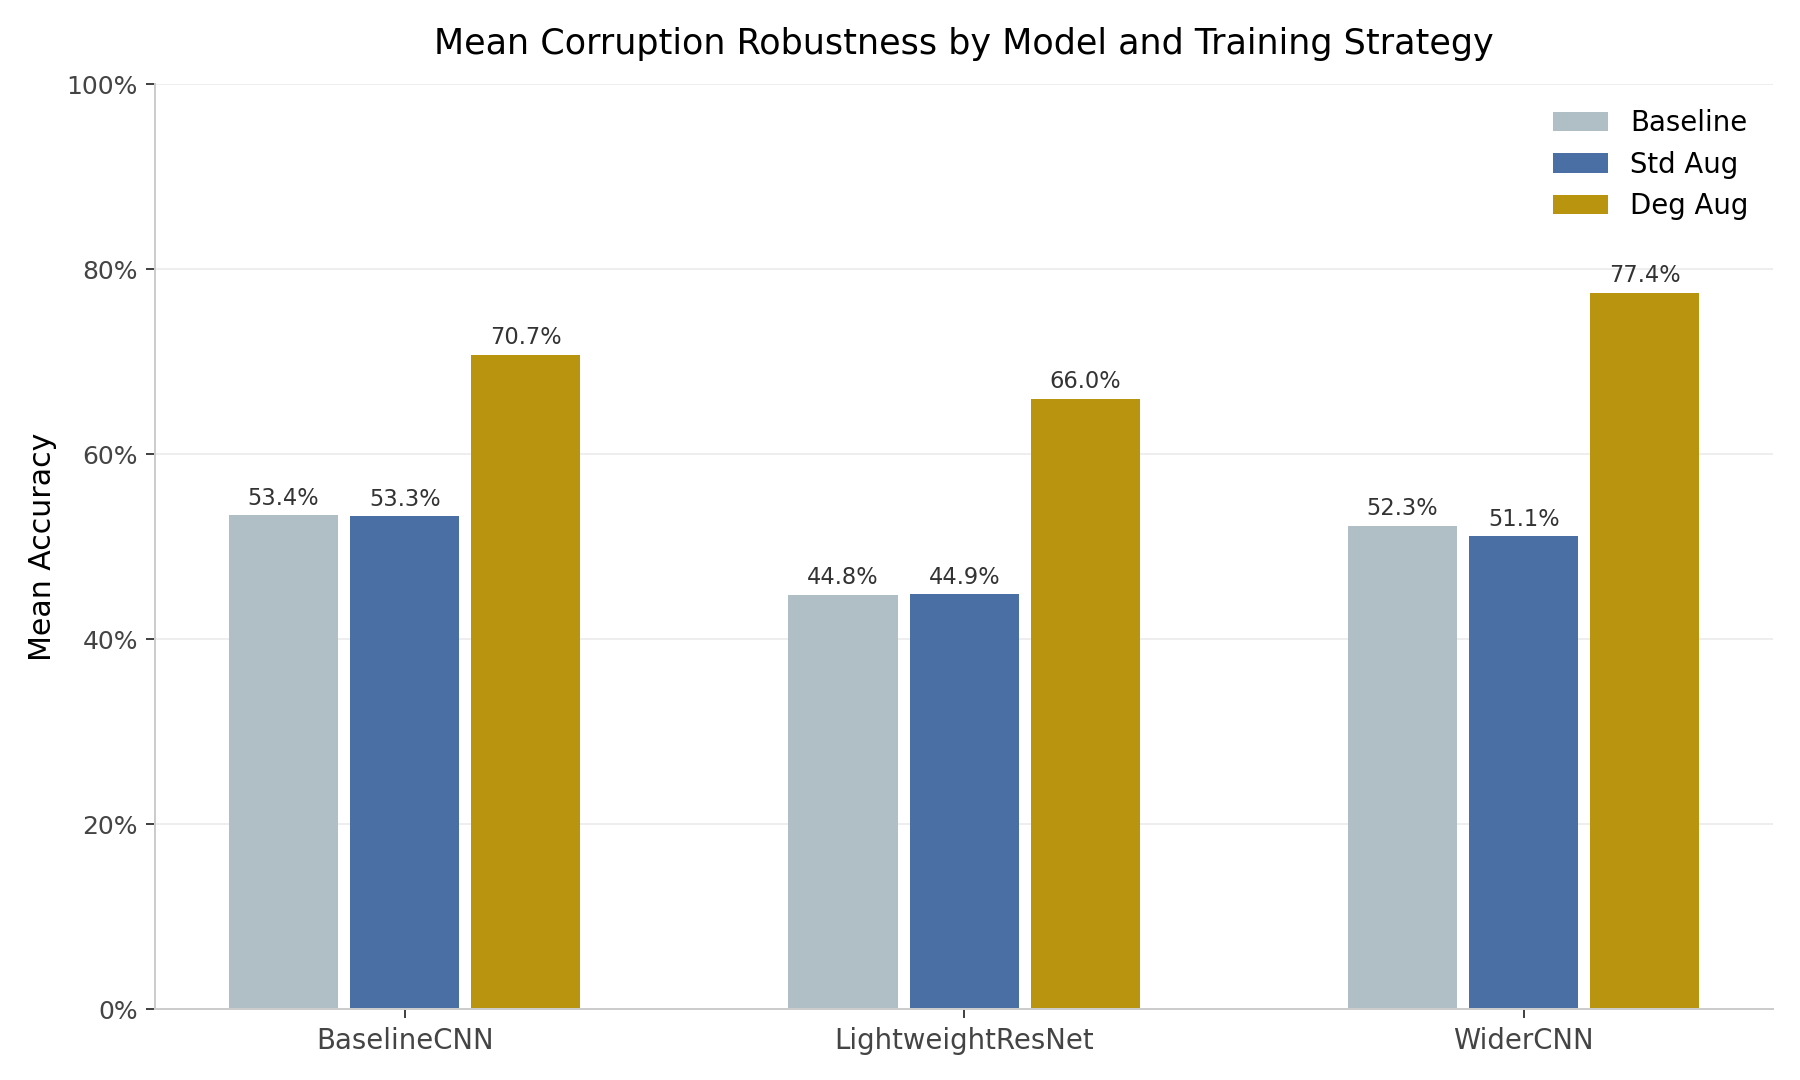
\includegraphics[width=\columnwidth]{plot2_model_strategy.png}
\caption{Mean corruption accuracy by model and training strategy, averaged across all 25 corruption conditions.}
\label{fig:model_strategy}
\end{figure}

\subsection{Per-Corruption Breakdown}

Table~\ref{tab:percorruption} and Fig.~\ref{fig:strategy_corruption} show mean accuracy per corruption type, averaged across all three models and all five severity levels. Gaussian noise is the most damaging corruption by a considerable margin: baseline and standard augmentation achieve only 0.302 and 0.261 mean accuracy respectively, while degradation-aware augmentation raises that to 0.626 --- more than doubling robustness. JPEG compression and brightness change are the most tolerable, with all three strategies exceeding 0.63. The gap between standard augmentation and degradation-aware augmentation is largest for Gaussian noise and smallest for JPEG compression, a pattern that holds consistently across individual models.

\begin{table}[h]
\caption{Mean Accuracy per Corruption Type (avg.\ over 3 models)}
\label{tab:percorruption}
\centering
\begin{tabular}{lccc}
\toprule
\textbf{Corruption} & \textbf{Baseline} & \textbf{Std Aug} & \textbf{Deg Aug} \\
\midrule
Gaussian Noise       & 0.302 & 0.261 & \textbf{0.626} \\
Gaussian Blur        & 0.478 & 0.480 & \textbf{0.724} \\
JPEG Compression     & 0.638 & 0.642 & \textbf{0.725} \\
Resolution Reduction & 0.455 & 0.465 & \textbf{0.735} \\
Brightness Change    & 0.634 & 0.640 & \textbf{0.759} \\
\bottomrule
\end{tabular}
\end{table}

\begin{figure}[h]
\centering
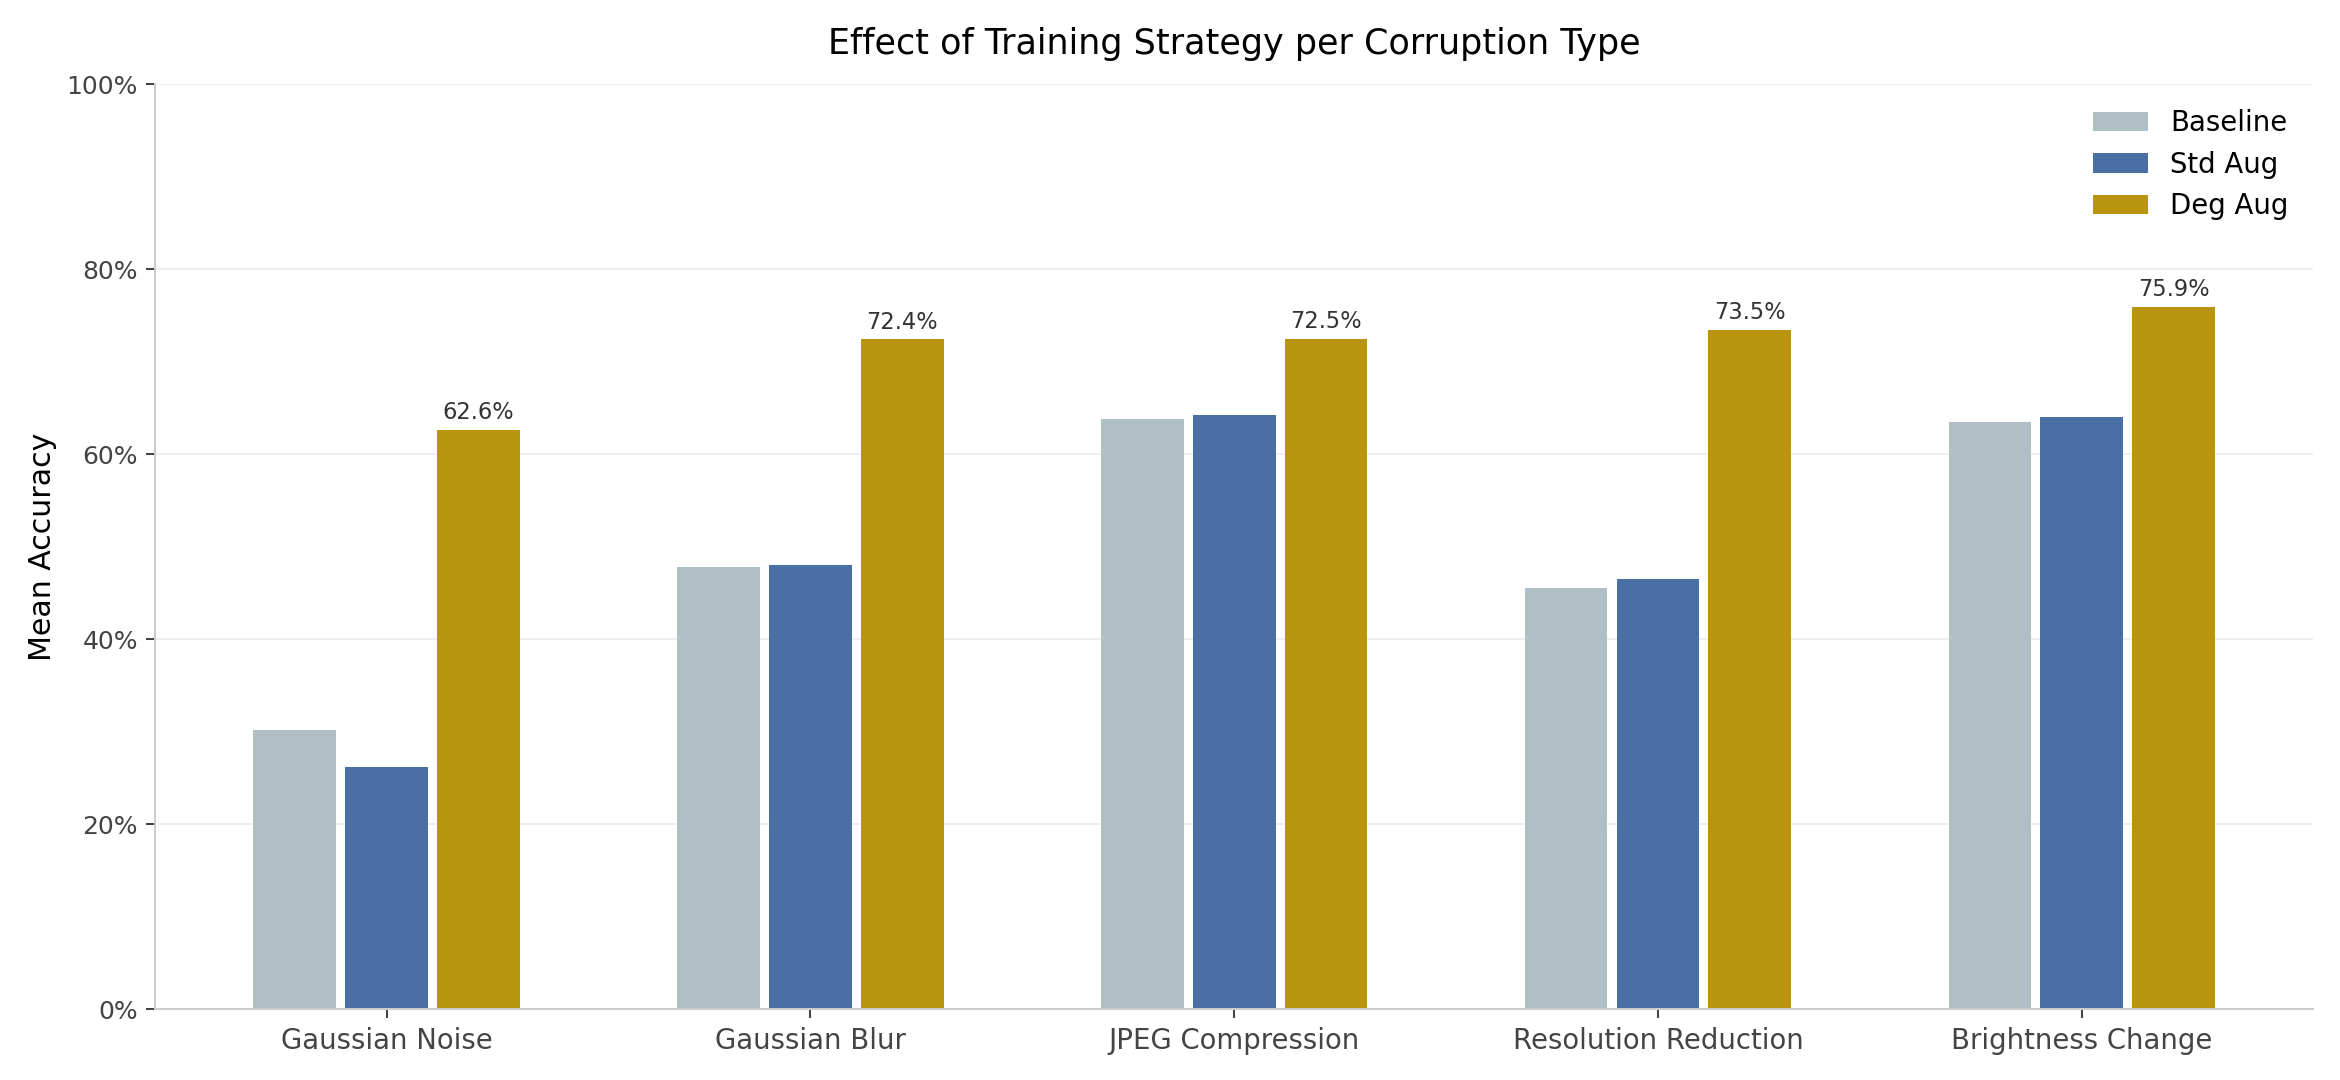
\includegraphics[width=\columnwidth]{plot3_strategy_per_corruption.png}
\caption{Effect of training strategy per corruption type, averaged across all three models and five severity levels.}
\label{fig:strategy_corruption}
\end{figure}

\subsection{Per-Severity Results}

Table~\ref{tab:severity} shows BaselineCNN accuracy at each severity level under unaugmented training. The degradation curves differ substantially across corruption types. Gaussian noise accuracy collapses quickly --- from 71.3\% at severity 1 to 14.3\% at severity 5, a drop of 57 percentage points. Gaussian blur follows a different pattern: accuracy stays above 79\% at severities 1--2, then falls sharply at severity 3 (43.7\%) before continuing to decline. JPEG compression is notably stable by comparison, degrading gradually from 76.2\% to 51.8\% across five levels. Resolution reduction shows a steep drop at severity 4 (32.6\%), suggesting a threshold effect once downsampling reaches $16{\times}16$ pixels. Brightness change behaves non-monotonically because levels 1--3 darken the image progressively while levels 4--5 switch to brightening; accuracy recovers from 32.4\% at severity 3 to 75.8\% at severity 4.

\begin{table}[h]
\caption{BaselineCNN Accuracy per Severity Level (Baseline Training)}
\label{tab:severity}
\centering
\begin{tabular}{lccccc}
\toprule
\textbf{Corruption} & \textbf{S1} & \textbf{S2} & \textbf{S3} & \textbf{S4} & \textbf{S5} \\
\midrule
Gaussian Noise       & 0.713 & 0.528 & 0.380 & 0.225 & 0.143 \\
Gaussian Blur        & 0.797 & 0.733 & 0.437 & 0.265 & 0.237 \\
JPEG Compression     & 0.762 & 0.725 & 0.689 & 0.625 & 0.518 \\
Resolution Reduction & 0.653 & 0.598 & 0.511 & 0.326 & 0.281 \\
Brightness Change    & 0.771 & 0.682 & 0.324 & 0.758 & 0.673 \\
\bottomrule
\end{tabular}
\end{table}

\section{Analysis and Validation}

\subsection{Research Objectives Evaluation}

Three research questions were posed at the outset. All three are answered by the experimental results, and the project objectives were met: a systematic, quantitative analysis of robustness trends across 25 corruption conditions and three training strategies was completed as planned, with results that speak directly to each question.

\textit{RQ1 --- How does performance change as image quality degrades?} Performance degrades substantially and non-uniformly. Gaussian noise causes the steepest decline across all models, with accuracy dropping below 20\% at severity 4 under unaugmented training. Blur and resolution reduction follow intermediate trajectories. JPEG compression is the most tolerable, suggesting that block-level compression artifacts are less disruptive to the features learned by these models than pixel-level noise. The degradation pattern is corruption-specific rather than a uniform function of severity, which has practical implications --- different deployment environments carry different failure risks.

\textit{RQ2 --- To what extent do low-cost strategies improve robustness?} Standard augmentation does not improve robustness in any meaningful way. Degradation-aware augmentation improves mean corruption accuracy by 17.3 percentage points for BaselineCNN, 21.2 for LightweightResNet, and 25.2 for WiderCNN, relative to unaugmented training. These are large gains achieved without changing model architecture or increasing parameter count. The cost is modest: a slight clean accuracy reduction for LightweightResNet and negligible cost for the other two models.

\textit{RQ3 --- Are gains from degradation-aware augmentation consistent across corruption types?} Largely yes, but with variation. The gains are largest for Gaussian noise (0.302 to 0.626 averaged over models) and smallest for JPEG compression (0.638 to 0.725). Even for JPEG, where baseline models already perform reasonably, degradation-aware augmentation provides an additional 8--9 percentage point improvement. Gains are consistent in direction across all five corruption types, which was the core question.

\subsection{Comparison with Existing Work}

The robustness gains observed here are meaningful but more modest than those reported in large-scale studies, which is expected given the constrained setting. Hendrycks et al.\ reported that AugMix achieves a mean corruption error of around 11.2\% on ImageNet-C for ResNet-50, representing a substantial improvement over standard training~\cite{hendrycks2020}. In this study, degradation-aware augmentation achieves mean corruption \textit{accuracy} of 66--77\% across models on CIFAR-10, which reflects a comparable directional improvement relative to baseline but cannot be compared directly due to dataset and architecture differences.

More directly relevant is the finding of Rusak et al., who showed that noise-based augmentation can generalize well across unseen corruptions~\cite{rusak2020}. The present results are consistent with that finding in one respect: degradation-aware augmentation, which includes noise during training, produces the largest gains under Gaussian noise. However, gains are also substantial for blur and resolution reduction, suggesting the approach is not purely noise-specific in this setting.

The finding that standard augmentation provides no robustness benefit is consistent with Mintun et al.'s analysis~\cite{mintun2021}, who showed that geometric transformations like flipping and cropping are perceptually dissimilar to pixel-level corruptions and therefore do not transfer robustness. The present results provide direct empirical confirmation of this mechanism in a lightweight, constrained setting where it had not been explicitly tested.

\subsection{Why Standard Augmentation Fails}

The near-zero benefit of standard augmentation is arguably the most practically useful finding in this study. Random flipping and cropping change the spatial layout of an image but leave pixel statistics intact. A model trained with these transformations learns some invariance to object position and orientation --- which is why clean accuracy improves --- but the distribution of pixel intensities, frequency content, and local texture statistics remains unchanged. When test images are corrupted by noise or blur, those statistics shift substantially. Standard augmentation provides no exposure to that kind of shift.

This is worth stating explicitly because standard augmentation is often described as a robustness technique in general terms. Based on these results, it is better understood as a regularization strategy that improves clean generalization without addressing input distribution shift of the kind that corruptions produce.

\subsection{Is Degradation-Aware Augmentation Trivially Expected to Win?}

A natural objection is that the gains from degradation-aware augmentation are simply expected: a model that sees corrupted images during training will obviously handle corrupted images at test time. That reasoning is not wrong, but it understates what the results show.

Standard augmentation also exposes the model to modified inputs --- yet provides no robustness benefit whatsoever. The critical difference is not that the model sees \emph{any} augmented data, but that it specifically sees the kinds of distribution shifts present at test time. Degradation-aware augmentation works because it aligns training perturbations with evaluation corruptions, consistent with Mintun et al.~\cite{mintun2021}, who showed robustness improvements correlate strongly with perceptual similarity between training and test perturbations. The contrast with standard augmentation is the finding, not the win by degradation-aware augmentation alone.

There is also a cost side to consider. Degradation-aware augmentation reduces clean accuracy for LightweightResNet by 4 percentage points, from 80.9\% to 76.9\%. For BaselineCNN the cost is under 1 point and for WiderCNN essentially zero. In settings where corruption robustness is important, the trade-off is clearly favorable for two of three models.

\subsection{Architecture and Robustness}

A recurring pattern across corruption types is that BaselineCNN is more robust to Gaussian noise than LightweightResNet under unaugmented training, despite having lower clean accuracy. At severity 1, BaselineCNN reaches 71.3\% under Gaussian noise compared to 54.0\% for LightweightResNet --- a gap of over 17 percentage points. This is counterintuitive. LightweightResNet uses residual connections, batch normalization, and global average pooling, all of which are generally expected to improve generalization.

One explanation is that global average pooling averages activations across all spatial positions. When noise corrupts every spatial location equally, this averaging distributes the noise effect uniformly across the representation rather than suppressing it. BaselineCNN uses max pooling, which selects the strongest activation in each spatial region and may retain some noise-tolerant selectivity. This interpretation is speculative but consistent with the texture-bias literature~\cite{geirhos2019}: networks that have not learned highly specialized feature detectors may respond more conservatively when their inputs are disrupted.

Architectural complexity does not automatically confer robustness. WiderCNN achieves the highest robustness under degradation-aware augmentation (77.5\%), and clean accuracy does correlate with robustness once training strategy is held constant. The relationship between model complexity and robustness is not monotonic under unaugmented training, which is the relevant finding.

\subsection{Limitations}

Several limitations of this study are worth acknowledging. First, and most importantly, models were evaluated only on the same five corruption types used during degradation-aware training. Whether these robustness gains transfer to entirely unseen corruptions --- such as elastic distortions, pixelation, fog, or motion blur --- remains untested. The results therefore speak to robustness within a known corruption set, not to generalization beyond it. This is a meaningful constraint on the scope of the conclusions.

Second, each augmented model was trained with a single random seed. For the unaugmented baseline, three seeds were used and the best was selected, which introduces a small selection bias in favor of the baseline models when comparing absolute numbers. The directional findings are unlikely to be affected, but the exact magnitude of robustness gaps should be interpreted with this in mind.

Third, all experiments are conducted on CIFAR-10 at $32{\times}32$ resolution. At this resolution, spatial features play a smaller role than at larger resolutions, and the behavior of global average pooling under noise may differ on higher-resolution datasets where feature maps retain more spatial structure. Conclusions about architectural robustness should not be assumed to transfer directly to larger-scale settings.

Finally, the brightness severity scale is non-monotonic by design --- levels 1--3 darken and levels 4--5 brighten --- which complicates direct comparison with other corruption benchmarks that use monotonically increasing severity scales. Results for brightness should be interpreted within the context of this scale definition rather than compared numerically to other studies.

\section{Discussion and Conclusion}

\subsection{Main Contributions}

This study set out to characterize robustness trends for lightweight CNNs under realistic image corruptions in a constrained training setting. Three contributions emerge from the results.

First, degradation-aware augmentation substantially improves corruption robustness across all three architectures, raising mean accuracy across 25 conditions by 17--25 percentage points relative to unaugmented training, with negligible or no clean accuracy cost for two of three models. Second, standard augmentation --- despite its widespread use and its genuine benefit for clean accuracy --- provides no meaningful robustness improvement. Mean accuracy differences between baseline and standard augmentation fall below 2 percentage points for all models and all corruption types. Third, architectural sophistication does not reliably predict corruption robustness. Under unaugmented training, a simple four-layer CNN outperforms a residual network with batch normalization and global average pooling on the most destructive corruption type tested.

\subsection{Key Findings}

Performance degrades non-uniformly across corruption types, with Gaussian noise causing accuracy drops of up to 57 percentage points at high severity levels while JPEG compression causes a more gradual 24-point decline. Standard augmentation does not address this degradation in any meaningful way. Degradation-aware augmentation provides consistent gains across all five corruption types, with the largest improvement for Gaussian noise and the smallest for JPEG compression --- a pattern consistent with the frequency-domain analysis of Yin et al.~\cite{yin2019}, since noise is a high-frequency corruption that training exposure directly addresses.

The finding that BaselineCNN outperforms LightweightResNet under noise without augmentation points to a specific mechanism: global average pooling, while effective for clean generalization, distributes noise uniformly across the feature representation rather than suppressing it. Max pooling retains more spatial selectivity under noise. Whether this effect holds on higher-resolution datasets or more complex architectures is an open question that warrants follow-up investigation.

\subsection{Implications}

In resource-constrained settings where architectural redesign is expensive or impractical, the choice of training strategy has a larger effect on corruption robustness than the choice of model. Standard augmentation should not be assumed to address input distribution shift --- it is primarily a regularization tool. Degradation-aware augmentation is a low-cost alternative that meaningfully improves robustness when the test-time corruption types are known in advance. The main caveat is that these gains are likely conditional on the match between training and test corruptions, consistent with prior work~\cite{mintun2021}. For deployment scenarios where the corruption types are unknown, more general robustness methods such as AugMix~\cite{hendrycks2020} may be preferable despite their higher training cost.

\subsection{Future Work}

Several directions follow naturally from these results. Testing generalization to unseen corruption types would directly address the primary limitation of this study. Combined corruptions --- noise and blur applied simultaneously, for example --- would better reflect real-world degradation conditions where multiple factors degrade image quality at once. Extending the evaluation to higher-resolution datasets such as CIFAR-100 or STL-10 would clarify whether the observed patterns hold beyond the $32{\times}32$ regime. Investigating whether the global average pooling noise-sensitivity hypothesis holds under controlled ablation experiments would put the architectural finding on firmer empirical ground. Finally, comparing degradation-aware augmentation against AugMix under matched compute budgets would situate these findings within the broader robustness literature more precisely.

\begin{thebibliography}{1}

\bibitem{hendrycks2019}
D.~Hendrycks and T.~Dietterich, ``Benchmarking neural network robustness to common corruptions and perturbations,'' in \textit{Int.\ Conf.\ on Learning Representations (ICLR)}, 2019. [Online]. Available: https://arxiv.org/abs/1903.12261

\bibitem{hendrycks2020}
D.~Hendrycks, N.~Mu, E.~D.~Cubuk, B.~Zoph, J.~Gilmer, and B.~Lakshminarayanan, ``AugMix: A simple data processing method to improve robustness and uncertainty,'' in \textit{Int.\ Conf.\ on Learning Representations (ICLR)}, 2020. [Online]. Available: https://arxiv.org/abs/1912.02781

\bibitem{mintun2021}
E.~Mintun, A.~Kirillov, and S.~Xie, ``On interaction between augmentations and corruptions in natural corruption robustness,'' in \textit{Advances in Neural Information Processing Systems}, vol.~34, 2021. [Online]. Available: https://arxiv.org/abs/2102.11273

\bibitem{geirhos2019}
R.~Geirhos, P.~Rubisch, C.~Michaelis, M.~Bethge, F.~A.~Wichmann, and W.~Brendel, ``ImageNet-trained CNNs are biased towards texture; increasing shape bias improves accuracy and robustness,'' in \textit{Int.\ Conf.\ on Learning Representations (ICLR)}, 2019. [Online]. Available: https://arxiv.org/abs/1811.12231

\bibitem{rusak2020}
E.~Rusak, L.~Schott, R.~S.~Zimmermann, J.~Bitterwolf, O.~Bringmann, M.~Bethge, and W.~Brendel, ``A simple way to make neural networks robust against diverse image corruptions,'' in \textit{Computer Vision -- ECCV 2020}, Cham: Springer, 2020, pp.~53--69. [Online]. Available: https://arxiv.org/abs/2001.06057

\bibitem{yin2019}
D.~Yin, R.~G.~Lopes, J.~Shlens, E.~D.~Cubuk, and J.~Gilmer, ``A Fourier perspective on model robustness in computer vision,'' in \textit{Advances in Neural Information Processing Systems}, vol.~32, 2019, pp.~13255--13265. [Online]. Available: https://arxiv.org/abs/1906.08988

\end{thebibliography}

\end{document}